\documentclass[conference, 11pt]{IEEEtran}
\IEEEoverridecommandlockouts

\usepackage{amsmath,amssymb,amsfonts}
\usepackage{algorithmic}
\usepackage{graphicx}
\usepackage{textcomp}
\usepackage{xcolor}
\usepackage{hyperref}
\usepackage{caption}
\usepackage[
    backend = biber,
    language = auto,
    style = numeric,
    sorting = none,
    block = space,
    hyperref = true,
    bibencoding = auto,
    giveninits = true,
    doi=false,
    isbn=false,
    alldates=short
]{biblatex}
\addbibresource{literature.bib}

\captionsetup{justification=centering,margin=0.5cm}

\def\BibTeX{{\rm B\kern-.05em{\sc i\kern-.025em b}\kern-.08em
    T\kern-.1667em\lower.7ex\hbox{E}\kern-.125emX}}
\begin{document}

\title{3DCV - Critical Driving Scenarios\\
{\small Generate critical driving scenarios in CARLA simulator and apply imitation learning to train a neural network}
}

\author{
    \IEEEauthorblockN{Christopher Klammt}
    \and
    \IEEEauthorblockN{Tobias Richstein}
    \and
    \IEEEauthorblockN{Julian Seibel}
    \and
    \IEEEauthorblockN{Karl Thyssen}
}

\maketitle

\begin{abstract}

\end{abstract}

\begin{IEEEkeywords}

\end{IEEEkeywords}

\section{Introduction}
Autonomous driving vehicles are a not just an idea for the more distant future, but rather a very current topic.
Not only Tesla, the company that dominates the news in this regard, is showing how far autonomous driving has come in the last years.
One crucial issue still lies in providing a stable and safe behavior in critical situations, especially in which traffic participants behave unexpectedly. 
The problem is that to robustly learn the appropriate behavior for these specific critical scenarios and to generalize using supervised learning a large amount of training data is needed.

In order to tackle this problem, our paper describes the development of a generator for such critical driving scenarios in the CARLA simulator.
These critical driving scenarios are mainly inspired by the report \citetitle{NHTSA:PreCrashScenarios} \cite{NHTSA:PreCrashScenarios} for the National Highway Traffic Safety Administration in the United States.
These contain scenarios such as avoiding an obstacle, lane changing with oncoming traffic or crossing traffic running a red light at an intersection (as shown in \autoref{fig:scenario-run_red_light}).

\begin{figure}[ht]
    \centering
    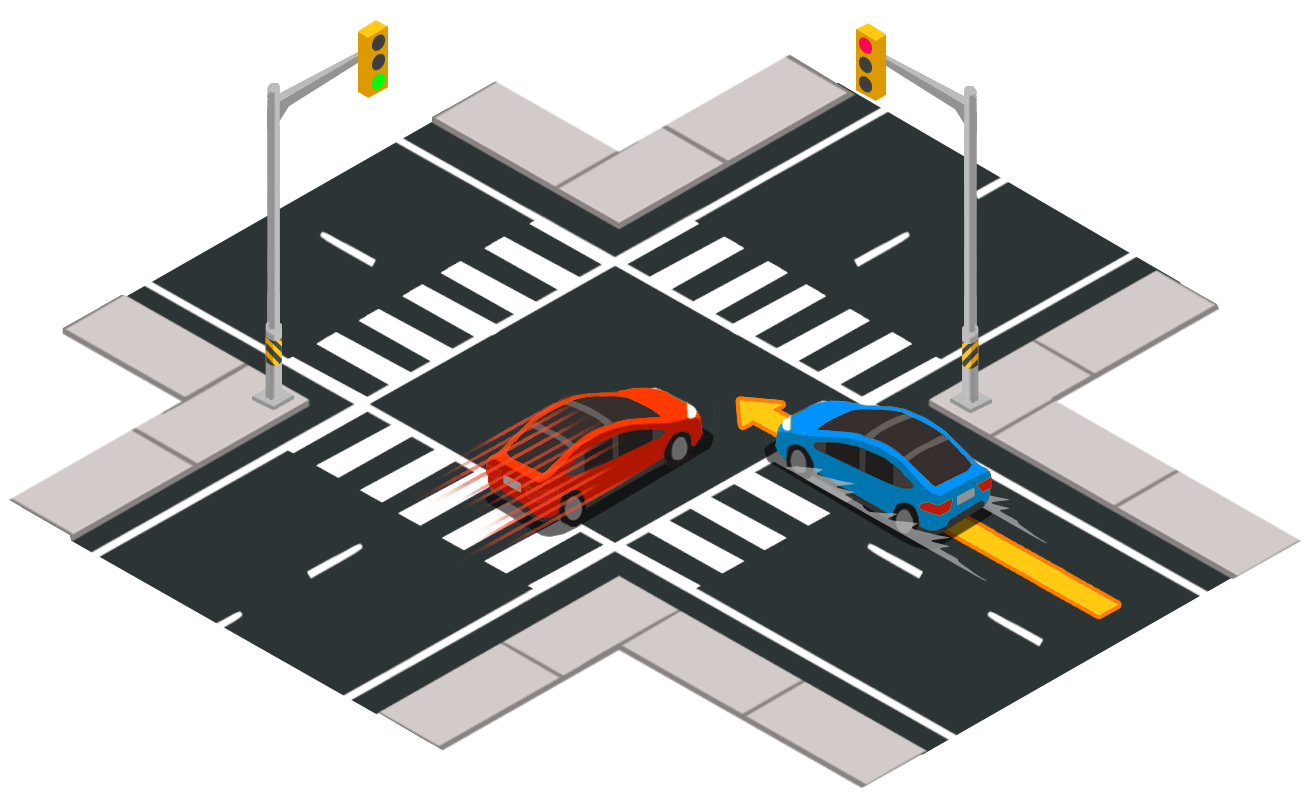
\includegraphics[width=0.7\linewidth]{figures/scenario-run_red_light.png}
    \caption{NHTSA scenario: Crossing traffic running a red light at an intersection \cite{CARLAChallenge:Scenarios}}
    \label{fig:scenario-run_red_light}
\end{figure}

Furthermore, after generating these different critical driving scenarios we utilize them to learn a robust model.
To do so imitation learning is used, in which an expert demonstrates the desired behavior in each critical situation and is then adopted by the model.

\section{Related Work}

\subsection{CARLA}
As presented by \citeauthor{Dosovitskiy17:CARLA}, CARLA is an open-source urban driving simulator for autonomous driving research \cite{Dosovitskiy17:CARLA}.
It enables handling different use cases within the general problem of driving, such as learning driving policies or training perception algorithms.
To control the simulation, e.g. changing weather, adding cars or pedestrians, an API is available in Python and C++.
CARLA consists of the simulator responsible for rendering etc. as well as multiple components, for example a traffic manager controlling the vehicles or a component handling the sensors.

\subsection{Critical driving scenarios}

Another component that works in unison with the CARLA simulator is the ScenarioRunner \cite{CARLA:ScenarioRunner}.
This is a module that makes it possible to define various traffic scenarios and execute them in the CARLA simulator.
These scenarios can be defined using Python or the OpenSCENARIO \cite{OpenScenario} standard.
The ScenarioRunner already contains some predefined Scenarios which are based on the critical driving scenarios as described in \citetitle{NHTSA:PreCrashScenarios} \cite{NHTSA:PreCrashScenarios}.

\subsection{Generating data in simulators}

In order to generate data it first is necessary to identify parameters that are to be adjusted and that should vary across the different entities.
The data generation can then be approached in different ways.
One possibility is to use a random statistical distribution of these parameters. 

Another way to go about data generation is to use learning-based methods to adjust the parameters of the simulator.
Such an approach was chosen by \citeauthor{DBLP:LearningToSimulate} and published in \citetitle{DBLP:LearningToSimulate} \cite{DBLP:LearningToSimulate}.
They proposed a reinforcement learning-based method to adjust the parameters of the synthesized data to maximize the accuracy of a model trained on that data.
A quite similar approach was chosen by \citeauthor{DBLP:Meta-Sim} \cite{DBLP:Meta-Sim} called Meta-Sim, which learns a generative model of synthetic scenes and modifies the attributes using a neural network.

\subsection{Imitation learning}

To learn a model based on labeled data some form of supervised learning is generally applied.
\citeauthor{Chen:LearningByCheating} propose a method called \citetitle{Chen:LearningByCheating} \cite{Chen:LearningByCheating}.
This is a two-stage method, in which first an agent is trained using privileged information.
In the second stage, the privileged agent acts as a teacher that trains a purely vision-based agent.

Another approach is \citetitle{Toromanoff_2020_CVPR} \cite{Toromanoff_2020_CVPR}. Here reinforcement learning is utilized to learn an optimal behavior policy based on a reward-function, effectively punishing wrong behavior such as leaving the track or running over pedestrians.

To train and manage the trainings of imitation learning networks jointly with evaluations on the CARLA simulator \citetitle{felipecode:coiltraine} \cite{felipecode:coiltraine} can be used.

\section{Generator for critical driving scenarios}

\subsection{Adjustable parameters}

CARLA and the ScenarioRunner enable us to adjust quite a few parameters, so that the generator can create a lot of diverse settings.
This includes the type and model of the car, which is steered by the learned agent, but more importantly of each and every other car.
This is important so that the model generalizes well, even if different cars are in it's field of vision.
Furthermore, to strain this point, we can also change the color of all cars, resulting in different RGB patterns perceived by the cars sensors.

Another parameter, that can be changed is the speed of the cars, which also has an impact on the behavior in critical situations.
The weather plays an important role, as it drastically changes what is perceived by sensors and also alters the effects of a certain behavior. For example rain does not only impair the video of the camera, but additionally lengthens the breaking distance.
These variables can all be adjusted rather easily, by just randomly picking a value from a predefined set.

The part of the configuration, which is more difficult to vary is with regards to further actors, such as pedestrians and other vehicles.
These have to be spawned somewhere and a behavior needs to be defined.
CARLA provides a list of possible spawn points across a map, but if we just choose these randomly, we cannot be sure, that the spawned car has an impact on our scenario.
Furthermore, the behavior of the cars is rather non-trivial.
Most importantly, the behavior of the car, which characterizes the critical scenario needs to well defined.
But apart from that, we also want vehicles in the background, that drive around somewhat automated.

\printbibliography

\end{document}
